\section{System Overview}\label{sec-arch}
In this section, we give an overview of the entire architecture of SVC.

\subsection{Problem Statment}
Using the notation defined in the previous section. 
Let $S$ be a materialized view defined by the relational expression $S_{def}$ a composition of operators defined in Section ?? applied to the database $\mathcal{D}$.
Now suppose the relations in $\mathcal{D}$ have been updated with the correponding set of delta relations $U = \{\Delta R_i\} \cup \{\nabla R_i\}$.
Let $\mathcal{D}'$ be the updated database and let $S'$ be the up-to-date view ($S_{def}$ applied to $\mathcal{D}'$).

\subsubsection{Problem 1. Sampling the Maintenance Plan: }
Define $\mathcal{M}(\mathcal{D},S_{def},S,U)$ \footnote{For brevity, we will drop the parameters when not ambiguous.} a maintenance strategy (be it incremental maintenance, full recomputation, or a mix) parametrized by the database, the view definition, the stale view, and the set of updates.
A maintenance is a relational expression the execution of which returns $S'$.
The only pre-condition on the maintenance plan is that it is composed of only the operations defined in the previous section. 

Given the relational expression $\mathcal{M}$, we apply the hash-sampling operator $\eta(\mathcal{M})$ and to maintain only a subset of the multiset $S'$.
With $\eta(\mathcal{M})$ as input, we return an optimized the execution of the sampled maintenance plan $\eta(\mathcal{M})^*$ to minimize computation.
This is achieved by a set of rules to pushing the sampling operation down the query tree of $\mathcal{M}$ allowing more operators to take advantage of the sampling. 
The result is a sampled maintenance plan which updates only a sample of the materialized view $\hat{S'} = \eta(\mathcal{M})$.

\subsubsection{Problem 2. Correction Plan: }
Given a query $q$ and an up-to-date sample created by the previous procedure $\hat{S'}$, we return a relational expression $C(q, S, \hat{S'}, O)$\footnotemark[2] which is a function of the query, the old view, the sampled up-to-date view, and the outlier index $O$. When the relational expression $C$ is executed the result $\hat{r}$ is an estimate of the true value $r$ which is defined as the limit of sampling operator to a 100\% sample.

Like similar restrictions in other sampled-based systems \cite{agarwalknowing}, there are restrictions on the queries $q$ on the view that we can answer. 
In this work, we primarily consider non-nested aggregate queries with simple predicates on a single view:
\begin{lstlisting} [mathescape]
SELECT $f(a)$ FROM View 
WHERE Condition(A);
\end{lstlisting}
We also consider correcting stale non-nested select queries of the following form with simple predicates:
\begin{lstlisting} [mathescape]
SELECT * FROM View 
WHERE Condition(A);
\end{lstlisting}
As with all sample estimates, for the estimates to be meaningful, the predicate should not be too selective.

\begin{table*}[ht!]
\caption{Query Result Semantics} % title of Table
\centering % used for centering table
\begin{tabular}{c c c c} % centered columns (4 columns)
\hline\hline %inserts double horizontal lines
Queries & Unbiased & Bounded Bias & Type of Bound \\ [0.5ex] % inserts table 
%heading
\hline % inserts single horizontal line
\sumfunc, \countfunc, \avgfunc & Yes & - & Optimal Analytical Via CLT \\ % inserting body of the table
\histfunc, \corrfunc, \varfunc, \covfunc & Yes & - & Empirical Via Bootstrap \\
\medfunc, \percfunc & No & Yes & Empirical Via Bootstrap \\
\maxfunc, \minfunc & No & No & Loose Probability Bound via Cantelli's Inequality \\
\texttt{f(DISTINCT)} & No & No & None in general \\ [1ex] % [1ex] adds vertical space
\hline %inserts single line
\hline
\texttt{SELECT *} & Yes & Yes & Optimal bound on result size 
\end{tabular}
\label{table:nonlin} % is used to refer this table in the text
\end{table*}

\subsection{Semantics of Query Results}
We should note that there is an implicit design tradeoff in the way we formulated this problem.
By sampling the maintenance plans, our approach is very general with respect to supported views.
On the other hand, we are restricted in the types of queries that we can run.
If we were to sample from the delta relations instead, this tradeoff would be flipped. 
We have a further discussion about this subtlty in Section ??.

A important concern of users is what are the semantics and guarantees on their corrected query results.
In Table ??, we list all of the aggregate queries supported by Apache HiveQL present a taxonomy of result semantics for these queries.
We will detail the corrections to these queries in Section \ref{correction}.

\subsection{Pratical Use and Implementation}
In implementation, SVC will work in conjunction with existing defered maintenance or re-calculation approaches.
We envision the scenario where materialized views are being refreshed periodically, for example nightly.
While maintaining the entire view throughout the day may be infeasible, sampling allows the database to scale the cost with the performance and resource constraints during the day.
Then, between maintenance periods, we can provide approximately up-to-date query results for some queries.

\subsection{Example Application: Log Analysis}
Without getting into the formal details, to illustrate our system and justify our argument about performance improvements, we use the following running example which is a 
simplified schema of one of our experimental datasets (Figure~\ref{example-1}).
Imagine, we are querying logs from a video streaming company. 
These logs record visits from users as they happen and grow over time.
We have two tables, \tbl{Log} and \tbl{Video}, with the following schema:

\begin{lstlisting}[mathescape]
Log(sessionId$\textrm{,}$ videoId$\textrm{,}$ responseTime$\textrm{,}$ userAgent)
Video(videoId$\textrm{,}$ title$\textrm{,}$ duration)
\end{lstlisting}
These tables are related with a foreign-key relationship between
Log and Video, and there is an integrity constraint that every log
record must link to one video in the Video table.

\begin{figure}[ht!] 
\centering
\vspace{-0.75em}
 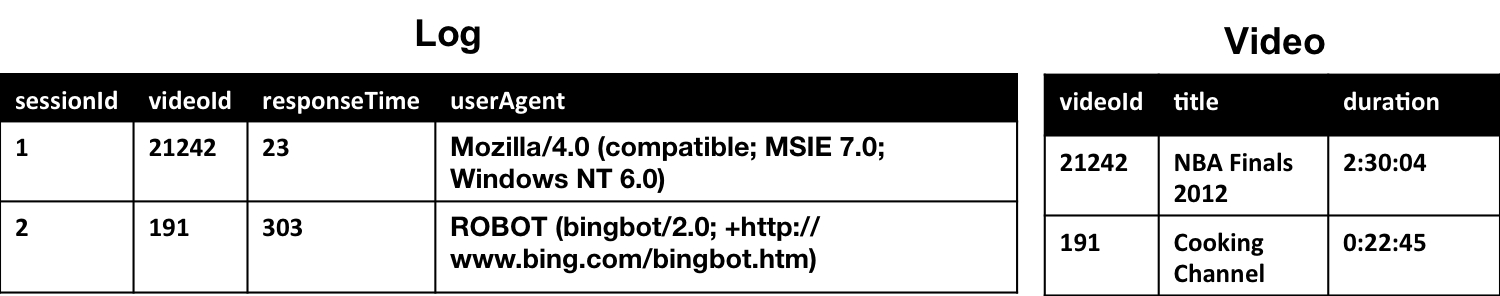
\includegraphics[width=\columnwidth]{figs/sample-clean-example.png}\vspace{-0.25em}
 \caption{A simplified log analysis example dataset. In this dataset, there are two tables: a fact table representing video views and a dimension table representing the videos.\label{example-1}}
\end{figure}

Consider the following example materialized view, which finds a count of the number of times the video's loading latency was greater than 10\% of the duration of the view:

\vspace{0.5em}

\begin{lstlisting} 
SELECT videoId, 
count(1) AS slowResponseTimes 
FROM Log, Video
WHERE Log.videoID = Video.videoID and
	  responseTime > .1*Video.duration
GROUP BY videoId;
\end{lstlisting}

The user wants to know how many videos repeatedly have slow responses.
\begin{lstlisting} 
SELECT COUNT(1)
FROM AggView
WHERE slowResponseTimes > 100;
\end{lstlisting}
Let us suppose the initial query result is $45$.
There now have been new log records inserted into the Log table making the old result stale.
For example, if our sampling ratio is 5\%, that means for 5\% of the videos (distinct videoID's) we refresh stale slowResponseTimes if necessary.
From this sample, we calculate how many new videos changed from a slowResponseTimes of less than 100ms to times greater than 100ms; let us suppose this answer is $2$.
Since our sampling ratio is 5\%, we extrapolate that $40$ new videos throughout the view should now be included in the count.
This means that we should correct the old result by $40$ resulting in the estimate of $85$.